% Chapter Template

\chapter{Introduction} % Main chapter title

\label{Chapter1} % Change X to a consecutive number; for referencing this chapter elsewhere, use \ref{ChapterX}

%----------------------------------------------------------------------------------------
%	SECTION 1
%----------------------------------------------------------------------------------------

\section{Motivation}

Deafness is considered to be the most prevalent impairment worldwide, affecting at least 278 million people \cite{Tucci2010}. However, current provisions for those who may struggle to fully hear and comprehend human speech in commercial settings is distinctly lacking. Cinemas routinely show only 2 or 3 showings a week with subtitles in the UK \cite{subtitledshows},  restricting the range of films and times that can be enjoyed, adding to the sense of exclusion experienced by disabled people. There are technologies available to provide captions for individual users\cite{dolbysubs}, but these rely on each institution having purchased these, and are far from universally available. Even those that do have them only provide them for a small selection of movies, 6/27 at one cinema chain in New Zealand \cite{hoyts}. Therefore, to ensure availability of these it is desirable to find methods that could be applied on the user-side so that subtitles can be made available in whichever context the user desires. Time stamped subtitle files are freely available as SubRip files (.srt file extension) that contain a series of text entries and associated start and stop times, but these rely on knowing the exact start time of a film so that the 2 files are synchronised. This is extremely difficult to achieve in a live setting where the exact commencement of the feature film is unclear, and the introduction of even a small time shift can make subtitle viewing an unwatchable experience. Hence, the demand arises to automatically synchronise a subtitle file using real time audio signals to locate the current position in a video.

\section{Background}

This problem was tackled in a laboratory setting\cite{Sabater_2017}, so that a user can synchronise audio and subtitle tracks for future viewing on a personal device. This method extracted and sampled the audio at 16kHz, extracted the features using the common automatic speech recognition (ASR) technique of splitting the signal into 20-40ms frames and extracting the Mel Frequency Cepstral Coefficients for each frame and using these as the predictive features. The subtitle track was then used to create a binary array indicating whether subtitles (and therefore human speech) occur in each corresponding frame to those used for MFCC, providing the target variable. A Recurrent Neural Network (RNN) was initially trained, a logical approach given the chronological nature of the data, but due to the fact that several frames must be used as input, the accuracy was limited to the duration of the number of input frames: if 10*0.05s samples are required, the accuracy is limited to 0.5s which is insufficient in practise. Therefore a Convolutional Neural Network (CNN) was trained, taking as input just 1 sample, with several one-dimensional convolutional layers followed by several dense layers to output an array containing the probabilities that human speech is present in each frame. Technically, it should be noted that since the presence of subtitles is the target variable, a subtitle- (rather than speech-) detector was built. Minimisation of the log loss function was then used to align the subtitles array with the probability array, the delay calculated and applied to the subtitle track; this loss function was chosen in order to maximise the accuracy by penalising false classifications. Using this process, after training the NN and hyperparameter tuning, the log-loss minimum is clearly defined \ref{loss_sabater}.
\begin{wrapfigure}{r}{0.5\textwidth} 
	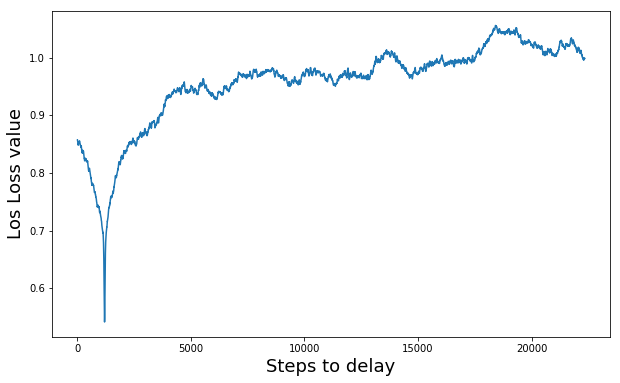
\includegraphics[width=0.4\textwidth]{log_loss_steps_sabater}
	\caption{Log loss plot when matching full audio to full subtitles}
	\label{loss_sabater}
\end{wrapfigure}
Using dynamic programming to take account of the fact that every step must be evaluated across the signal, this process took 45 seconds for a tv show and 2 minutes for a film, the whole process using CPU’s. 
This approach is promising and formed the basis upon which this study was formed. There were key differences in the aim that require further study in order to implement this in a live setting.  Since this was performed on the recorded data rather than a live recording, the signals are pure and contain no significant noise, and so a model that could handle such settings needed to be identified. Furthermore, there would be more uncertainty in the start times of the film which would need to be accounted for – search can commence from the beginning and match the 2 full arrays since the aim is to match the full sound track with the subtitle track (with less concern for excessive processing time), whereas in real time, access to the sound track would occur incrementally as new audio is recorded. The Sabater study was informal, with the results released as a blog post and so lacked a rigorous (or at least reporting of the) approach and testing environment, with no account of the relative complexities and possible different approaches that could be taken. \newline

A similar approach was adapted in \cite{Ortega2009} in order to align a draft script with a live presentation which loosely followed this but often presented changes in the script and its chronology (insertions, substitutions and deletions). To do so, 12 order MFCC’s were used again, and “normalised energy coefficient augmented by the corresponding delta and delta-delta coefficients information as features”(p2), but an ASR engine formed of “continuous HMM's [Hidden Markov Models] with context dependent acoustic units, where each unit is modelled with a 16 component Gaussian Mixture Model with diagonal covariance matrices” was used. The HMM’s enable sequence data to be modelled and are not constrained in the same way as RNN’s that must take multiple sequential samples in order to predict a sample, thereby reducing the accuracy achievable. This was a more ambitious objective in that the audio had not been prerecorded and so to compare the audio to the subtitles, the MFCC’s were compared to a phoneme network in order to identify utterances and therefore alignment of the tracks. In addition, this system substituted automatically generated subtitles when no script was available due to insertions.
This model achieved an accuracy of up to 100\% on newscasts that adhered strictly to the script and naturally dropped to 30\% when the programme became unscripted. In addition, due to the preprocessed nature of the scripts the latency was deemed to be negligible. 
Another approach has been implemented \cite{Campbell1996} In which audio is generated from text by Text To Speech (TTS) systems and this is used to synchronise the text and audio. %This is a very promising idea and in the context of this paper’s problems would eliminate the requirement to have the film audio for training, and only the srt. Therefore the aim will be to extend the study to evaluate this method in the noisy setting.